\documentclass[a4paper]{article}
\usepackage[utf8]{inputenc}
\usepackage[spanish, es-tabla, es-noshorthands]{babel}
\usepackage[table,xcdraw]{xcolor}
\usepackage[a4paper, footnotesep = 1cm, width=20cm, top=2.5cm, height=25cm, textwidth=18cm, textheight=25cm]{geometry}
%\geometry{showframe}

\usepackage{tikz}
\usepackage{amsmath}
\usepackage{amsfonts}
\usepackage{amssymb}
\usepackage{float}
\usepackage{graphicx}
\usepackage{caption}
\usepackage{subcaption}
\usepackage{multicol}
\usepackage{multirow}
\setlength{\doublerulesep}{\arrayrulewidth}
\usepackage{booktabs}
\usepackage{mathrsfs,amsmath}
\usepackage{hyperref}
\hypersetup{
    colorlinks=true,
    linkcolor=blue,
    filecolor=magenta,      
    urlcolor=blue,
    citecolor=blue,    
}

\newcommand{\quotes}[1]{``#1''}
\usepackage{array}
\newcolumntype{C}[1]{>{\centering\let\newline\\\arraybackslash\hspace{0pt}}m{#1}}
\usepackage[american]{circuitikz}
\usetikzlibrary{calc}
\usepackage{fancyhdr}
\usepackage{units} 

\graphicspath{./Imagenes}

\pagestyle{fancy}
\fancyhf{}
\lhead{22.05 ASSD}
\rhead{Mechoulam, Lambertucci, Rodriguez, Londero}
\rfoot{Página \thepage}

\begin{document}
\section{Simulaciones Básicas}

Se simularon las funciones descritas en la Tabla (\ref{fn})

\begin{table}[H]
\centering
\begin{tabular}{@{}c@{}}
\toprule
Función \\ \midrule
$A\cdot Cos(2\pi \cdot 1.5kHz \cdot t)$ \\
Triangular simétrica 1.5kHz de pico $V_{MAX}$ \\
3/2 Seno amplitud VMAX 1.5kHz \\ \bottomrule
\end{tabular}
\caption{Funciones a simular}
\label{fn}
\end{table}

Se determinó que el valor máximo de amplitud de entrada al sistema es de $5V$ el cual es el mínimo entre los dos valores limitantes: Máxima entrada al CD4066 y límite mínimo de distorsión. Además, los límites de tensión de alimentación recomendados son 18V de la hoja de datos del CD4066.

Para hallar los valores óptimos de $A$, $F_s$ y $DT$ se simuló utilizando \textit{LTSpiceXVII} las curvas de entrada y salida del sistema variando simultáneamente los valores de las tres variables, previamente fijando los rangos de variación de las variables. Estos rangos son de $1V$ a $5V$ para $A$,
 $21kHz$ (para cumplir con el doble de la frecuencia de corte del filtro recuperador) a $25kHz$ (límite del oscilador) y de $5\%$ (límite del oscilador) a $50\%$ (limite por consigna) para el duty cycle. Finalmente, se utilizó el siguiente script en \textit{Python} para hallar el valor de las tres variables tal que la distorsión a la salida respecto a la entrada sea la mínima, computando la correlación entre las dos señales.

\begin{figure}[H]
\centering
\scalebox{0.75}{
\lstinputlisting{Python/spiceanal.py}
}
\end{figure}

Se obtuvieron los siguientes resultados.:

\begin{figure}[H]
\centering
\begin{subfigure}{\linewidth}
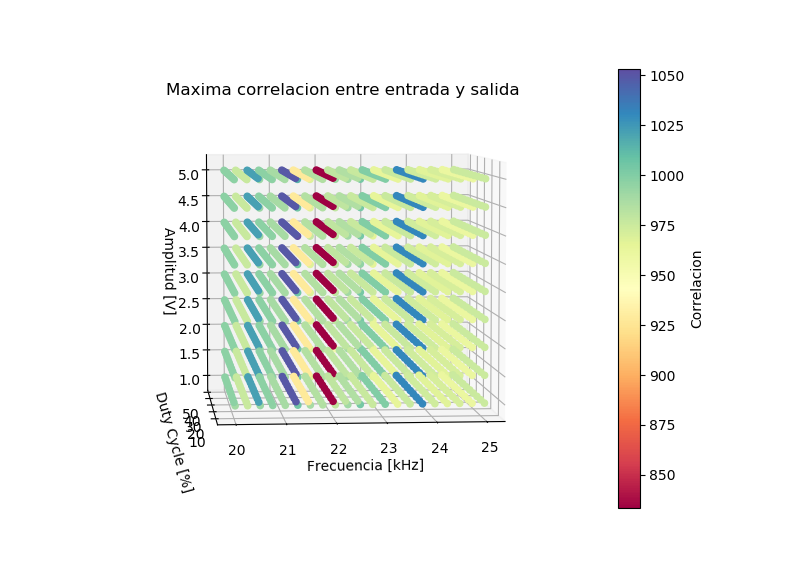
\includegraphics[width=\linewidth]{ImagenesEjercicio6/scatter_sh_seno.png}
\caption{Scatterplot de las simulación.}
\end{subfigure}

\begin{subfigure}{\linewidth}
\[A = 5V \ F_s = 22000Hz \ DT = 25\%\]
\caption{Parámetros para la menor distorsión.}
\end{subfigure}
\label{seno_sh}
\caption{Resultados experimentales de la simulación para \textbf{senoidal con S\&H}.}
\end{figure}

\begin{figure}[H]
\centering
\begin{subfigure}{\linewidth}
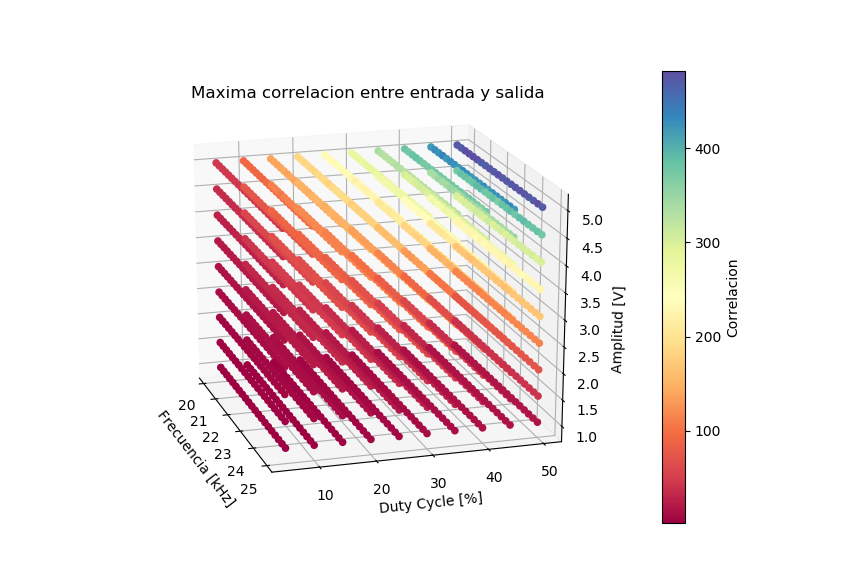
\includegraphics[width=\linewidth]{ImagenesEjercicio6/scatter_llave_seno.png}
\caption{Scatterplot de las simulación.}
\end{subfigure}

\begin{subfigure}{\linewidth}
\[A = 5V \ F_s = 21250Hz \ DT = 50\%\]
\caption{Parámetros para la menor distorsión.}
\end{subfigure}
\label{seno_llave}
\caption{Resultados experimentales de la simulación para \textbf{senoidal con llave analógica}.}
\end{figure}

\begin{figure}[H]
\centering
\begin{subfigure}{\linewidth}
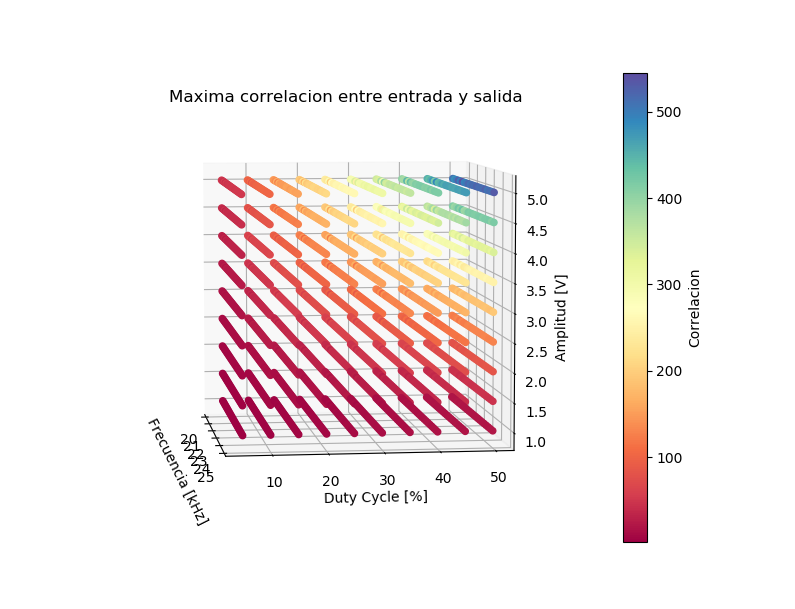
\includegraphics[width=\linewidth]{ImagenesEjercicio6/scatter_llave_triang.png}
\caption{Scatterplot de las simulación.}
\end{subfigure}

\begin{subfigure}{\linewidth}
\[A = 5V \ F_s = 23750Hz \ DT = 50\%\]
\caption{Parámetros para la menor distorsión.}
\end{subfigure}
\label{triang_llave}
\caption{Resultados experimentales de la simulación para \textbf{triangular con llave analógica}.}
\end{figure}

\begin{figure}[H]
\centering
\begin{subfigure}{\linewidth}
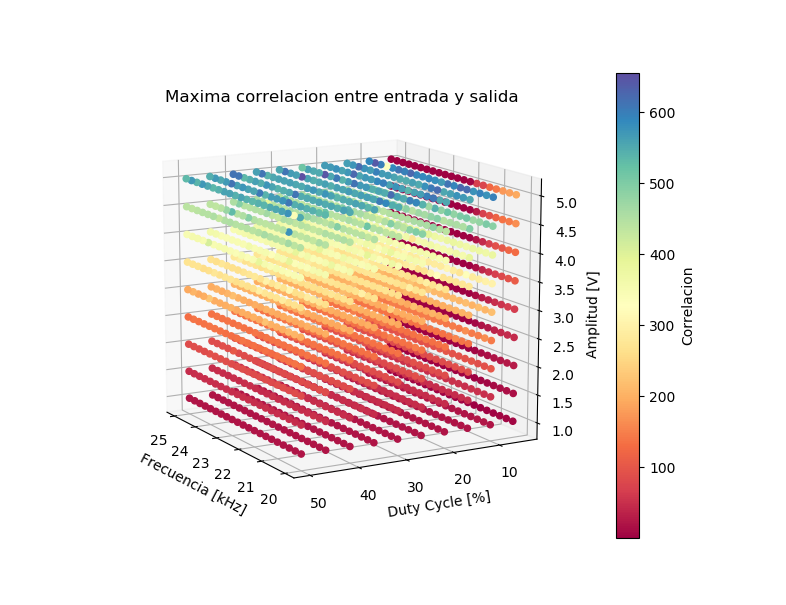
\includegraphics[width=\linewidth]{ImagenesEjercicio6/scatter_sh_triang.png}
\caption{Scatterplot de las simulación.}
\end{subfigure}

\begin{subfigure}{\linewidth}
\[A = 5V \ F_s = 24000Hz \ DT = 30\%\]
\caption{Parámetros para la menor distorsión.}
\end{subfigure}
\label{triang_sh}
\caption{Resultados experimentales de la simulación para \textbf{triangular con S\&H}.}
\end{figure}

\begin{figure}[H]
\centering
\begin{subfigure}{\linewidth}
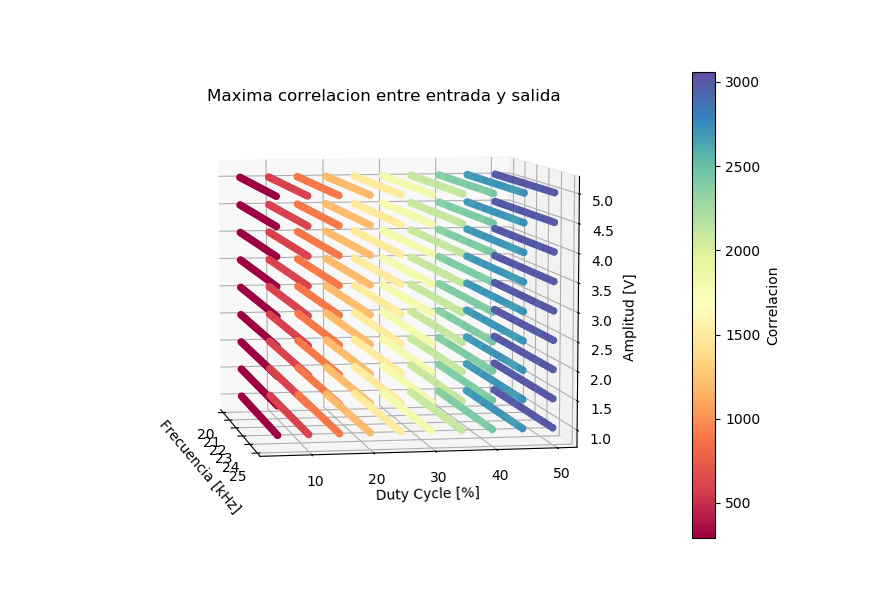
\includegraphics[width=\linewidth]{ImagenesEjercicio6/scatter_llave_sen32.png}
\caption{Scatterplot de las simulación.}
\end{subfigure}

\begin{subfigure}{\linewidth}
\[A = 1V \ F_s = 23500Hz \ DT = 50\%\]
\caption{Parámetros para la menor distorsión.}
\end{subfigure}
\label{sen32_llave}
\caption{Resultados experimentales de la simulación para \textbf{seno 3/2 con llave analógica}.}
\end{figure}

\begin{figure}[H]
\centering
\begin{subfigure}{\linewidth}
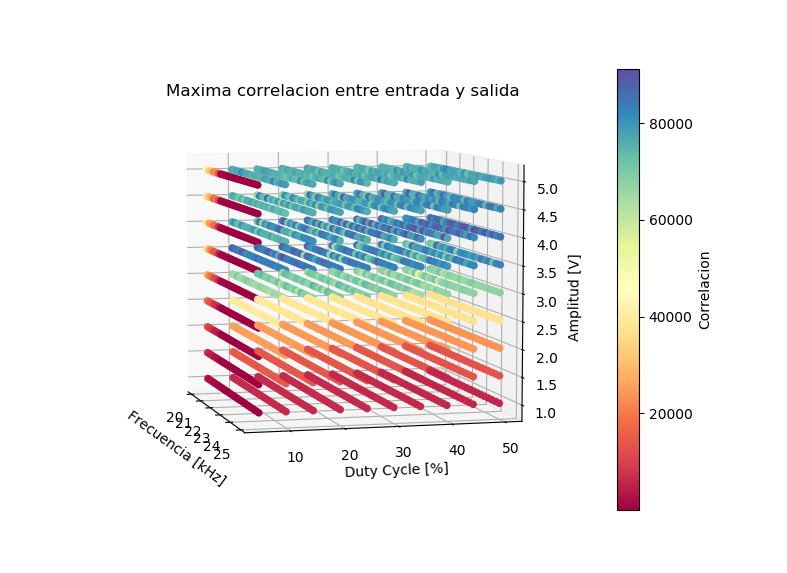
\includegraphics[width=\linewidth]{ImagenesEjercicio6/scatter_sh_sen32.png}
\caption{Scatterplot de las simulación.}
\end{subfigure}

\begin{subfigure}{\linewidth}
\[A = 1.5V \ F_s = 20000Hz \ DT = 5\%\]
\caption{Parámetros para la menor distorsión.}
\end{subfigure}
\label{sen32_sh}
\caption{Resultados experimentales de la simulación para \textbf{seno 3/2 con S\&H}.}
\end{figure}

Finalmente, se recopilan los resultados para cada tipo de señal y sistema en la Tabla (\ref{tab:res}).
\begin{table}[H]
\begin{tabular}{@{}ccccccc@{}}
\toprule
Parámetro & Seno S\&H & Seno Llave & Triangular S\&H & Triangular Llave & Seno3/2 S\&H & Seno3/2 Llave \\ \midrule
Amplitud & 5V & 5V & 5V & 5V & 1.5V & 1V \\
Frecuencia de sampleo & 22000Hz & 21250Hz & 24000Hz & 23750Hz & 20000Hz & 23500Hz \\
Duty Cycle & 25\% & 50\% & 30\% & 50\% & 5\% & 50\% \\ \bottomrule
\end{tabular}
\label{tab:res}
\caption{Resultados experimentales de los parámetros del sistema para obtener menor distorsión.}
\end{table}

\subsubsection{Simulaciones con Python}
Se utilizó el framework de \textbf{GNURadio} para programar cada módulo del sistema encerrado en una interfaz gráfica, la cual brinda la posibilidad de visualizar tanto la señal en tiempo como su espectro en cada nodo del sistema en el mismo momento. Se puede elegir entre señales sinusoidales, triangulares, 3/2 seno o moduladas AM como entrada, señales cuyo estudio es de interes.

\subsubsection{Simulaciones con LTSpice}
Para ambos sistemas, tanto con la llave analógica seleccionada como para el Sample and Hold elegido, se realizaron las simulaciones de las funciones en la Tabla (\ref{fn}) con los parámetros del sistema que resultan en la menor distorsión según los resultados experimentales detallados en la Tabla (\ref{tab:res}).

%\begin{figure}[H]
%\centering
%\scalebox{0.9}{
%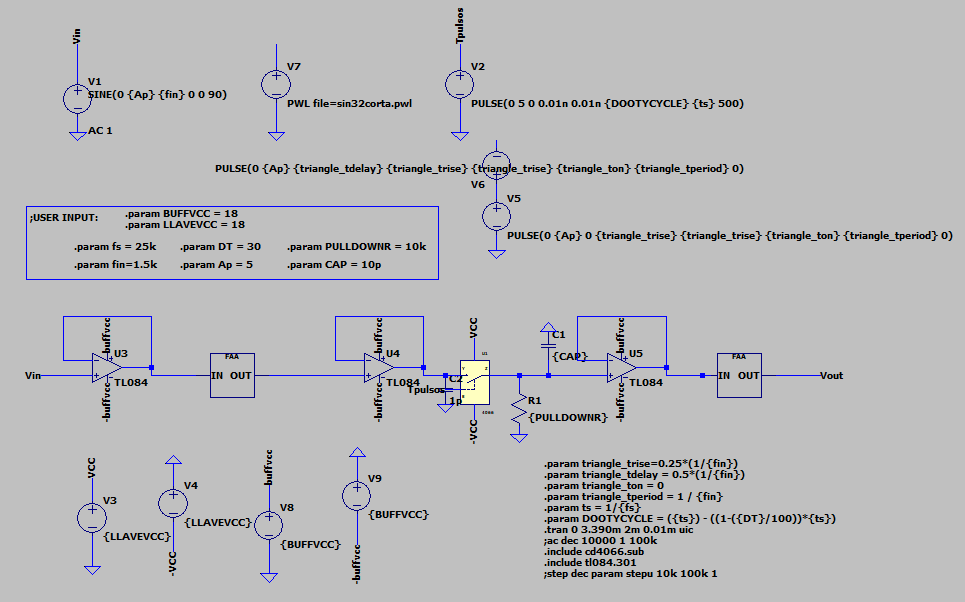
\includegraphics[width=\textwidth]{ImagenesEjercicio6/SIMULACIONLLAVE.png}
%}
%\caption{Esquema de simulación para el sistema con llave analógica.}
%\end{figure}
%
%\begin{figure}[H]
%\centering
%\scalebox{0.9}{
%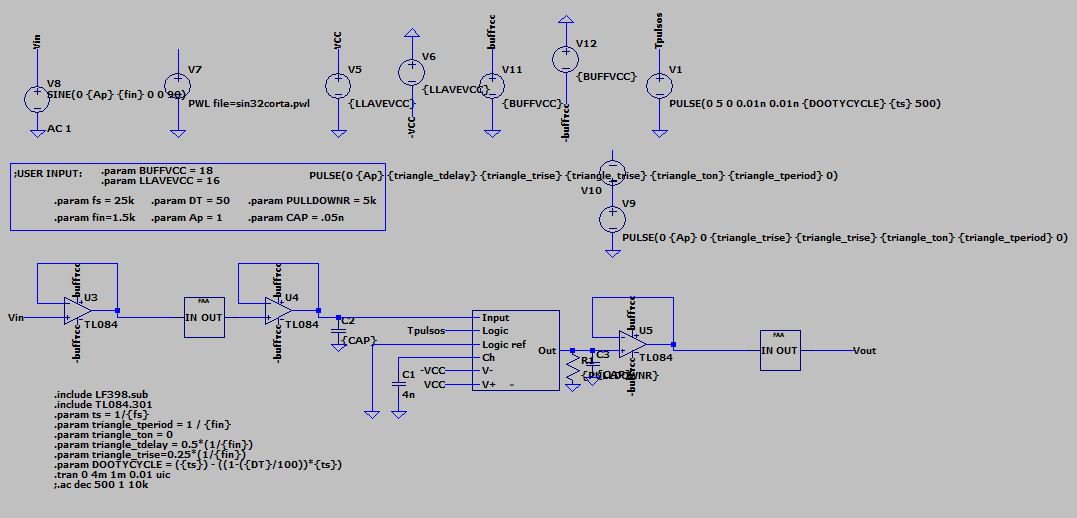
\includegraphics[width=\textwidth]{ImagenesEjercicio6/SIMULACIONSH.png}
%}
%\caption{Esquema de simulación para el sistema con Sample and Hold.}
%\end{figure}

\textbf{Senoidal con S\&H}

Se calculó para la señal senoidal muestreada con sample and hold con $5V$ de amplitud, $22000Hz$ de frecuencia de muestreo y duty cycle del $25\%$ mostrada en la Figura (\ref{fig:senollave}) un $93,21\%$ de potencia recuperada. 

\begin{figure}[H]
\centering

\includegraphics[width=\textwidth]{ImagenesEjercicio6/pend.jpg}
\caption{Comparación temporal entre entrada y salida del sistema.}
\end{figure}

\textbf{Senoidal con llave analógica}

Se calculó para la señal senoidal muestreada con llave analógica con $5V$ de amplitud, $21250Hz$ de frecuencia de muestreo y duty cycle del $50\%$ mostrada en la Figura (\ref{fig:senollave}) un $21,48\%$ de potencia recuperada. 

\begin{figure}[H]
\centering

\includegraphics[width=\textwidth]{ImagenesEjercicio6/pend.jpg}
\caption{Comparación temporal entre entrada y salida del sistema.}
\label{fig:senollave}
\end{figure}

\textbf{Triangular con S\&H}

Se calculó para la señal triangular muestreada con sample and hold con $5V$ de amplitud, $24000Hz$ de frecuencia de muestreo y duty cycle del $30\%$ mostrada en la Figura (\ref{fig:senollave}) un $101,05\%$ de potencia recuperada. 

\begin{figure}[H]
\centering

\includegraphics[width=\textwidth]{ImagenesEjercicio6/pend.jpg}
\caption{Comparación temporal entre entrada y salida del sistema.}
\end{figure}

\textbf{Triangular con llave analógica}

Se calculó para la señal triangular muestreada con llave analógica con $5V$ de amplitud, $23750Hz$ de frecuencia de muestreo y duty cycle del $50\%$ mostrada en la Figura (\ref{fig:senollave}) un $27,60\%$ de potencia recuperada. 

\begin{figure}[H]
\centering

\includegraphics[width=\textwidth]{ImagenesEjercicio6/pend.jpg}
\caption{Comparación temporal entre entrada y salida del sistema.}
\end{figure}

\textbf{Seno 3/2 con S\&H}

Se calculó para la señal seno 3/2 muestreada con sample and hold con $1.5V$ de amplitud, $20000Hz$ de frecuencia de muestreo y duty cycle del $5\%$ mostrada en la Figura (\ref{fig:senollave}) un $102,35\%$ de potencia recuperada. 

\begin{figure}[H]
\centering

\includegraphics[width=\textwidth]{ImagenesEjercicio6/pend.jpg}
\caption{Comparación temporal entre entrada y salida del sistema.}
\end{figure}

\textbf{Seno 3/2 con llave analógica}

Se calculó para la señal seno 3/2 muestreada con llave analógica con $1V$ de amplitud, $23500Hz$ de frecuencia de muestreo y duty cycle del $50\%$ mostrada en la Figura (\ref{fig:senollave}) un $32,59\%$ de potencia recuperada. 

\begin{figure}[H]
\centering

\includegraphics[width=\textwidth]{ImagenesEjercicio6/pend.jpg}
\caption{Comparación temporal entre entrada y salida del sistema.}
\end{figure}

Nuevamente, se realizaron las mismas simulaciones variando...

\textcolor{red}{\textbf{Aclarar bajo qué condiciones, es el punto 6b.}}

\end{document}